% Dissertation template for the Geophysics programs of the University of
% Liverpool.
%
% This document sets the configuration and assembles the individual chapters
% (stored in separate .tex files). See the declaration.tex file for
% instructions on including scanned signature.

% Fill these in and they will be set throughout the document
\newcommand{\Name}{Aidan Hernaman}  % Note that you can use any Unicode character
\newcommand{\Degree}{Master of Science in the subject of Geophysics and Geology}
\newcommand{\Title}{Estimating the accuracy of Moho depth estimates from gravity inversion}

\documentclass[11pt,a4paper,oneside]{book}
% Full Unicode support for non-ASCII characters
\usepackage[utf8]{inputenc}
% Typographical rules for English
\usepackage[english]{babel}
% Handling figures in PNG, JPG, PDF, etc
\usepackage{graphicx}
% Better and more extensive maths
\usepackage{amsmath}
% Set the borders of the page
\usepackage[width=150mm,top=40mm,bottom=30mm,headsep=10mm,headheight=5mm]{geometry}
% Include links and metadata in PDFs
\usepackage[pdftex,colorlinks=true]{hyperref}
% Define command to insert month name and year as date
\usepackage{datetime}
% Nice styling for headers and footers
\usepackage{fancyhdr}
% To control the style of section titles
\usepackage{titlesec}
% Add the bibliography to the table of contents
\usepackage[nottoc,chapter]{tocbibind}
% Formatting the bibliography
\usepackage[round]{natbib}
% To insert dummy text into this template. Can be removed.
\usepackage{lipsum}

% Define a date format that is just the month and year
\newdateformat{monthyear}{\monthname[\THEMONTH], \THEYEAR}

% Customize how Chapter headings are displayed
\titleformat{\chapter}[display]{\normalfont\bfseries\centering}{\vspace{-2cm}\LARGE Chapter \thechapter}{5pt}{\Huge}

% Setup metadata for the PDF and link colour
\hypersetup{
    pdftitle={\Title},
    pdfauthor={\Name},
    pdfsubject={Dissertation submitted for the degree of \Degree{}},
    linkcolor=black,
    citecolor=black,
    filecolor=black,
    urlcolor=blue
}

% Set fancy headers
\usepackage{fancyhdr}
\pagestyle{fancy}
\fancyhf{}
\lhead{\fontsize{10pt}{0}\selectfont\itshape \nouppercase\leftmark}
\chead{}
\rhead{\fontsize{9pt}{0}\selectfont \thepage}
\cfoot{}
\renewcommand{\headrulewidth}{0pt}
%\renewcommand{\chaptermark}[1]{\markboth{#1}{}}

% Increase the line spacing
\renewcommand{\baselinestretch}{1.5}

\begin{document}

  % Gather all of the .tex files for individual sections into a single
  % document. To add text and edit, open the individual files added with the
  % "\include{}" command.

  \pagestyle{plain}

  % You don't need to edit the cover, it will be generated from the variables
  % set at the very top of this document.
  % Cover page for the dissertation. Uses variables defined in the main
% dissertation.tex document. No need to edit things here.

%\addtolength{\topmargin}{-3in}

\thispagestyle{empty}

\begin{figure}[t!]
  \begin{center}
    
\includegraphics[width=0.7\textwidth]{figures/university-of-liverpool-logo.eps}
  \end{center}
\end{figure}

\vspace*{3cm}

\begin{center}
  \textbf{\LARGE \Title{}}
  \\[10mm]
  {\Large by}
  \\[10mm]
  {\Large \Name}
  \\
  \vfill
  \begin{minipage}[t]{0.7\textwidth}
    A dissertation submitted to the
    Department of Earth, Ocean, and
    Ecological Sciences,
    University of Liverpool, in partial fulfilment of
    the requirements for the degree of
    \Degree{}.
  \end{minipage}
  \\[3cm]
  \monthyear\today
\end{center}


  \frontmatter

  % You need to edit the declaration to include an image of your signature. See
  % the declaration.tex file for instructions.
  % Official declaration page that is required. The date is automatically set
% when the PDF is generated. Place a PNG file of your signature in the
% "figures" folder called "signature.png" (this exact name!). DON'T ADD THIS TO
% THE GIT RESPOSITORY!

\section*{Declaration}

\vspace{10mm}

I, \Name{}, confirm that the work submitted in this dissertation is my own, and
that appropriate credit has been given where reference is made to the work of
others.
\\[8mm]
\noindent Signature:

% To add your signature, place the "signature.png" file in the "figures"
% folder and uncomment the line below (remove the leading %).

\begin{figure}[h]
  %\includegraphics[width=50mm]{figures/signature.png}
\end{figure}

\noindent Date: \today

\newpage


  \section*{Acknowledgements}

First of all, I'm extremely grateful to Leonardo Uieda for being my supervisor for this Masters Project. I would also like to thank Eleanor Dacre and Lisa Palmer for their comments on the paper which helped improve the quality of this thesis.


  % Add your abstract to the "abstract.tex" file. DO THIS PART LAST. It's
  % easier to write the abstract in the end (and do a good job of it).
  \section*{Abstract}

For a long time, models of the Moho discontinuity have been created from a variety of different methods including gravitational and seismological studies. However, very few of these models developed have uncertainty estimates, this is especially the case where there is limited seismic data available. In areas such as South America and Africa due to the economic and environmental challenges, over vast regions of the continent, there are little to no seismic point estimates. For these areas to have relevant Moho models either gravitational data needs to be used or the seismic data has to be interpolated; there is no way to tell how accurate these methods are to attaining a true Moho depth model. To determine a method's accuracy a method of cross-validation specifically repeated random sub-sample validation will be used to quantify errors on a gravitationally derived model of South America with the help of seismic point estimates. The results from this cross-validation will evaluate the accuracy of gravitational models in regions where there is no seismic data to compare it to. Additionally, for regions where the model significantly underestimates the Moho depth in comparison to the seismic data, there is likely an unmodelled mass present. The Paraná Basin, South America is thought to have large igneous intrusions resulting in a shallower Moho than expected. In this study, these intrusions will be modelled in an attempt to decrease the errors on the Moho model currently used. The cross-validation gives an indication that the specific model used has a reasonably small misfit from the point estimates but that the size of the error may vary geographically across South America as the error values attained are an average for the whole model.




  % Table of contents and lists of figures and tables are automatically
  % generated (yay!)
  \tableofcontents
  \listoffigures

  \pagestyle{fancy}

  \mainmatter

  % These are the actual chapters of your dissertation. Add your text, figures,
  % tables, etc to these .tex files.
  \chapter{Introduction}

YOUR INTRODUCTION. The citations and bibliography are automatically handled by
BibTeX and the \texttt{natbib} package. Place the bibliographic information for
the references in the \texttt{references.bib} file and then cite your
references in the text (see below). The References section will be generated
automatically. To get the bibliographic information for papers, use the
\url{https://www.doi2bib.org/} website (DOIs are unique identifiers for
scientific publications, datasets, etc; you can find them in the paper PDFs or
publisher websites).

This is how you make citations: in the text \cite{Parker1973} or with
parenthesis \citep{Parker1973}. See
\url{https://www.overleaf.com/learn/latex/Natbib_citation_styles} for more
information.

The following is just filler text.

\lipsum[1-10]

  \chapter{Data and Methodology}

To accurately obtain a model of the Moho depth one must first remove all other effects that contribute to overall gravitational values recorded over an area (see Figure~\ref{fig:gravity-correction}). This is achieved through removing the scalar gravity of an ellipsoidal reference Earth (the Normal Earth) and then the removal of all other effects. Initially, though the effect of the Normal Earth needs to be removed from the same point as to where the gravity observation was made and is calculated from the closed-form solution in \cite{Li2001a}. The value obtained here is called the gravity disturbance and can be seen in equation~\ref{eq:gravity_disturbance} below.
\begin{equation}
  \mathbf{\delta}(\mathbf{P}) =
    {g}(\mathbf{P}) -
    \mathbf{\gamma}(\mathbf{P})
  % Label used to reference the equation in the text.
  \label{eq:gravity_disturbance}
\end{equation}

\begin{figure}[h]
  \begin{center}
    % Width can be set to particular size (10cm) or relative to the page size,
    % like 0.5\textwidth (for half page) or \textwidth (for full page).
    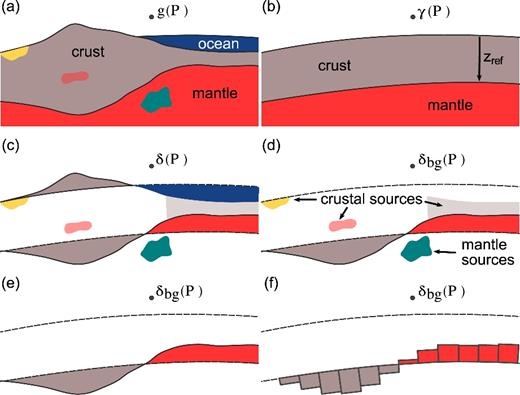
\includegraphics[width=0.7\textwidth]{figures/gravity-correction}
  \end{center}
  \caption{
    Step by step stages of the removal of gravitational effects. (a) The measured gravity at point P$(g(P))$ with reference to the Earth. (b) The Normal Earth and normal gravity at P$(\gamma(P))$. (c) Removal of density anomalies e.g. oceans and topography to get $(\delta(P))$ the gravity disturbance. (d) The crust and mantle sources left after obtaining the Bouguer disturbance $(\delta_{bg}(P))$ by removing topography. (e) Assuming there are no unmodelled masses the remaining signal is the Moho and its corresponding depth. (f) Discretization of the anomalous Moho into tesseroids. Grey tesseroids have a negative density contrast while red ones have a positive contrast. After \cite{Uieda2016}.
  }
  % Label used to reference the figure in the text.
  \label{fig:gravity-correction}
\end{figure}
The gravity disturbance is still not a direct result of the change in density associated with the Moho discontinuity but also an amalgamation of topography with reference to the normal ellipsoid, variations of density in the crust (e.g. sedimentary basins and igneous intrusions), anomalies below the upper mantle, and mass deficiency due to the oceans. The effects of topography and sedimentary basins are removed through a topography correction in equation~\ref{eq:topography_correction}.
\begin{equation}
  \mathbf{\delta_{bg}}(\mathbf{P}) =
    \mathbf{\delta}(\mathbf{P}) -
    {g_{topo}}(\mathbf{P})
  % Label used to reference the equation in the text.
  \label{eq:topography_correction}
\end{equation}
This is the method used in \cite{Uieda2016} and assumes that the effects of other crustal and mantle sources are negligible, and after this correction, the gravitational values attained are purely a result of the density variations on either side of the Moho discontinuity. Seeing as the data is obtained for a sufficiently large area (South America) this correction for topography amongst other things is calculated using tesseroids as part of a spherical Earth approximation. Tesseroids (Figure~\ref{fig:tesseroids}) are spherical prisms that are used in place of rectangular prisms as they account for the curvature of the Earth. Effects of the tesseroids are calculated using a GLQ integration presented in \cite{Asgharzadeh2007} and improved upon in \cite{Uieda2015} through the adaptive discretization scheme.
\begin{figure}[h]
  \begin{center}
    % Width can be set to particular size (10cm) or relative to the page size,
    % like 0.5\textwidth (for half page) or \textwidth (for full page).
    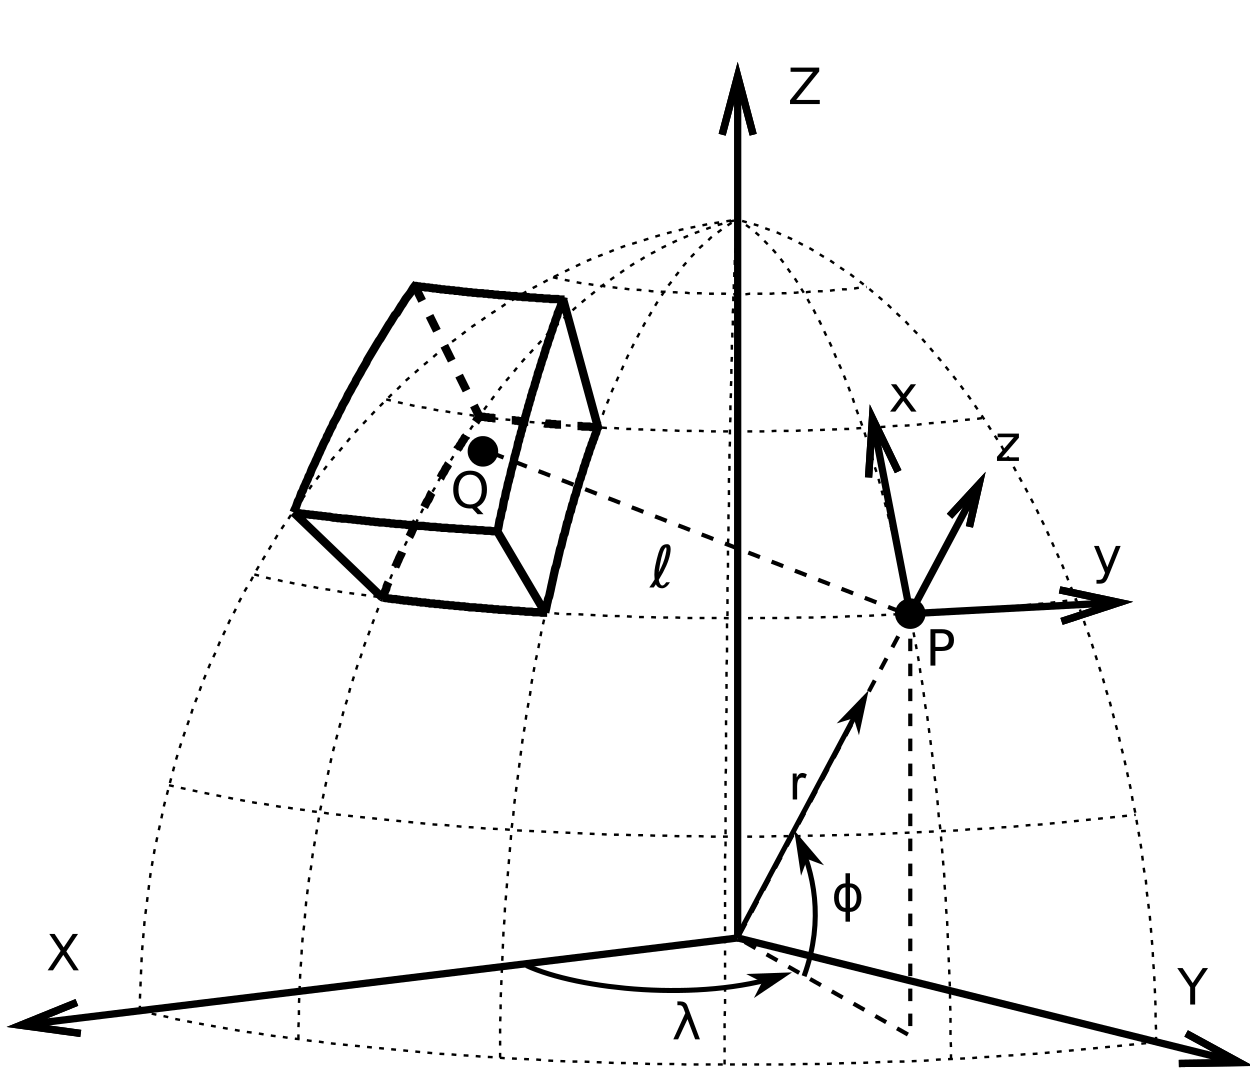
\includegraphics[width=0.6\textwidth]{figures/tesseroid-coord-sys}
  \end{center}
  \caption{
   Sketch of a tesseroid system with geocentric coordinates (X Y Z). Gravitational observations are made at point P with respect to its local north-orientated coordinate system (x y z). From \cite{Uieda2015}.
  }
  % Label used to reference the figure in the text.
  \label{fig:tesseroids}
\end{figure}
\section{Overview of the methodology from Uieda (2017)}
As the cross-validation to estimate uncertainty in the model is implemented as part of the code used in the \cite{Uieda2016} paper the method in calculating the model is largely similar. For context, an overview of this method will be given but for more detail see \cite{Uieda2016}.
Upon the calculation of the Bouguer disturbance from the removal of topography, sediments etc. the forward model is parameterized by discretizing the anomalous Moho onto tesseroids. The forward model aims to calculate the difference between the Normal Earth Moho and the true Moho depth, and depending on which is shallower will result in either a positive (red) or negative (grey) density contrast displayed by the colour of the tesseroids, Figure~\ref{fig:gravity-correction}. The overall absolute value of the density contrast is a certain parameter, this produces a nonlinear problem with the equation~\ref{eq:forward_problem}.
\begin{equation}
  \mathbf{d} =
    f(\mathbf{p})
  % Label used to reference the equation in the text.
  \label{eq:forward_problem}
\end{equation}
Where $d$ is the data vector, $p$ is the parameter vector containing Moho depths, and $f$ is the non-linear function.
Leading on to the inverse problem the parameter vector is estimated using least-squares that reduces the misfit to the data, equation~\ref{eq:least_squares}.
\begin{equation}
  \mathbf{\phi}(\mathbf{p}) =
    {[\mathbf{d}^o - \mathbf{d}(\mathbf{p})]}^T
    [\mathbf{d}^o - \mathbf{d}(\mathbf{p})]
  % Label used to reference the equation in the text.
  \label{eq:least_squares}
\end{equation}
Where $d^o$ is the observed gravity data, the equation means that this is a non-linear inverse problem, but we can calculate the parameters using optimization, where a perturbation vector $\Delta p^0$ is iterated until a minimum is reached which leads to the value of $\phi(p)$.
The optimization of the least-squares estimate however is not enough for estimating the relief associated with the Moho and needs regularization in the form of a first-order Tikhonov regularization \cite{Tikhonov1977} to ensure smoothness in the model and avoid unstable solutions in Moho depth, to provide a realistic model \cite{Silva2001b}, see equation~\ref{eq:regularization} below.
\begin{equation}
  \mathbf{\theta}(\mathbf{p}) =
    \mathbf{p}^T\mathbf{R}^T\mathbf{R}\mathbf{p}
  % Label used to reference the equation in the text.
  \label{eq:regularization}
\end{equation}
$R$ a matrix composed of first-order differences between Moho depths. This along with the least-squares estimate leads to an inverse problem that is solved by minimising the goal function, equation~\ref{eq:goal_function},
\begin{equation}
  \mathbf{\Gamma(p)} =
    \mathbf{\phi(p)} + \mathbf{\mu}\mathbf{\theta(p)}
  % Label used to reference the equation in the text.
  \label{eq:goal_function}
\end{equation}
$\mu$ is the regularization parameter that helps control the fit to the observed data and the smoothness.
After the rearrangement and substitution of equations, we arrive at a linear equation system that can calculate the update ($\Delta p$) with reference to the Normal Earth Moho,
\begin{equation}
  [\mathbf{\mathbf{A}^k}^T\mathbf{A}^k + \mathbf{\mu}\mathbf{R}^T\mathbf{R}] \mathbf{\Delta}\mathbf{p}^k =
    \mathbf{\mathbf{A}^k}^T [\mathbf{d}^o - \mathbf{d}(\mathbf{p}^k)] - \mathbf{\mu}\mathbf{R}^T\mathbf{R}\mathbf{p}^k
  % Label used to reference the equation in the text.
  \label{eq:linear_equation_system}
\end{equation}
Where $Ak$ is the Jacobian matrix, and $\Delta p^k$ is the parameter perturbation vector.
Bott's method \cite{Bott1960} calculates the thickness of a sedimentary basin based on gravitational data, the method is iterative so recalculates a new vector of basement depths from the previous calculation until a value where the residuals (equation numerator) fall below the noise level, see equation~\ref{eq:bott_method}.
\begin{equation}
  \mathbf{\Delta}\mathbf{p}^k =
    \mathbf{d}^o - \mathbf{d}(\mathbf{p}^k) /
    {2}\mathbf{\pi}{G}\mathbf{\Delta}\mathbf{\rho}
  % Label used to reference the equation in the text.
  \label{eq:bott_method}
\end{equation}
Where $\Delta p$ is the density contrast between the sediment and the reference density, and $G$ is the gravitational constant (6.67x10-11 $m^{-3} kg^{-1} s^{-2}$). However, \cite{Silva2014} showed that Bott's method can be written as,
\begin{equation}
  \mathbf{A} =
    {2}\mathbf{\pi}{G}\mathbf{\Delta}\mathbf{\rho}\mathbf{I}
  % Label used to reference the equation in the text.
  \label{eq:special_bott}
\end{equation}
and the main advantage to this is that this method does not need the solution of the equation system, but rather a constant diagonal matrix, $A$. This scales the model depths to fit the gravitational data.
For calculating the depth to the Moho \cite{Uieda2016} uses Bott's method in the inversion process and adapts it onto a spherical coordinate system using tesseroids. Stating in this paper that this method retains the efficiency of Bott's method while accounting for the stability problem previously present in the method. Following this step, the final part of the method involves calculating the hyperparameters (regularization parameter $\mu$, Moho density-contrast $\Delta p$, and depth of the Normal Earth Moho $z_{ref}$) which will be used in the inversion process. The calculation of the regularization parameter is through a method of holdout cross-validation from \cite{Hansen1992} and from this optimal regularization value, the other two hyperparameters (Moho density contrast $\Delta p$, and depth of the Normal Earth Moho $z_{ref}$) can be calculated. The main way these parameters are calculated is by finding the smallest Mean Square Error (MSE) through a cross-validation method which compares known Moho depths from seismic point estimates to calculated ones from the hyperparameters and picks the values with the smallest associated MSE.
\section{Implementation of cross-validation in error estimation}
Cross-validation (CV) often used for large data sets in order to see how well the model produced from said data set performs independently (i.e. when there is no data to base the model on). The result of cross-validation is often an MSE or mean square error value which is the accuracy of the new predicted independent model. It is often the goal of the cross-validation in the first place, and how this can be minimised. For many cases of CV, the data set is split up into a training and testing set with the training set being used to find the best solution or model attained from the smallest cross-validation value while the testing (validating) set is kept separate. It is then compared to the model created from the training set to get an idea of the size of errors, and how well a model will perform for a completely independent set. The cross-validation procedure also helps prevent overfitting of the model or selection bias where some points tend to skew the overall model more than others. And in order to minimise these problems the most, the process is repeated multiple times with different training and testing sets along with the variation in the size of these subsets.
Many types of CV are relevant for different case-specific things, although mostly the methods are split into two main types: exhaustive and non-exhaustive. Exhaustive CV is where all possible combinations of separating the full data into training and testing sets are used leading to a limited number of iterations that can be run. This method often works best for small volumes of data as with larger sets the computational time becomes uneconomical and an overall waste of time. Non-exhaustive CV does not use all possible combinations but rather a large enough number of iterations to be considered representative of the full data set.
For this method in particular a procedure of non-exhaustive repeated random sub-sampling validation also known as the Monte Carlo method. It works by as the name states repeatedly selecting a random selection of the data into a training and testing set, demonstrated in Figure~\ref{fig:RRSSV},
\begin{figure}[h]
  \begin{center}
    % Width can be set to particular size (10cm) or relative to the page size,
    % like 0.5\textwidth (for half page) or \textwidth (for full page).
    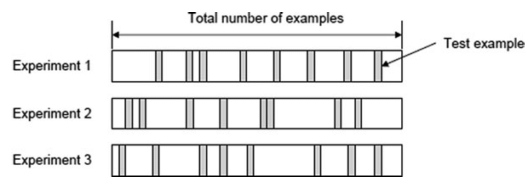
\includegraphics[width=0.8\textwidth]{figures/RRSSV}
  \end{center}
  \caption{
   Procedure of repeated random sub-sample validation with the data split into different training (white) and testing (grey) sets for each iteration. After \cite{unknown}.
  }
  % Label used to reference the figure in the text.
  \label{fig:RRSSV}
\end{figure}
with the sizes of each set being determined by the user. The training data is used to find the best model or solution with the associated lowest cross-validation score, and this then being compared to the testing or validating set to find the associated errors on the model. The procedure used here is similar but not to be confused with the exhaustive counterpart leave-p-out cross-validation which is the exact same process except it uses all combinations of the data, which hasn't been used here as random sampling is easier to implement. The data used here is seismic point data that is compared to a gravitationally derived moho model from selected hyperparameters. All the different models from different hyperparameter combinations are weighed up against a training set of seismic point estimates to find the model with the smallest variance or best match to these point estimates. It is then compared to the rest of the seismic data "held back" to find the Mean Square Error (MSE) and subsequently the Root Mean Square Error (RMSE), which is the average uncertainty of the model in kilometres. With 100 iterations per size and there being 3 sizes of training sets each being the closest integer value to fractions 2/3, 3/4, and 4/5 of the full data this would lead to a large enough proportion of all possible combinations to attain a representative insight to how well the model performs for an independent set. The full data consists of 937 seismic point estimates from \cite{Assumpo2013}, of which the locations can be seen in Figure~\ref{fig:seismic_locations},
\begin{figure}[h]
  \begin{center}
    % Width can be set to particular size (10cm) or relative to the page size,
    % like 0.5\textwidth (for half page) or \textwidth (for full page).
    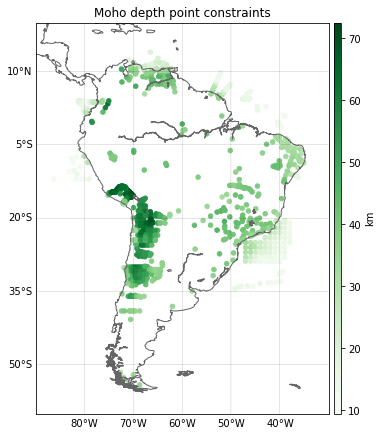
\includegraphics[width=0.5\textwidth]{figures/Seismic-locations}
  \end{center}
  \caption{
   Location and depth of seismic point estimates from \cite{Assumpo2013}. There are 937 total point estimates.
  }
  % Label used to reference the figure in the text.
  \label{fig:seismic_locations}
\end{figure}
meaning that the different training subset sizes are 625, 703 and 750, respectively. The training size always has to make up a larger proportion of the full data than the validating set as the model initially attained is representative of the overall data and hence the results of the MSE calculation is significant. This is supported by \cite{Berrar2019} who stated that 70-90\% of the full data should be part of the training set to be considered useful.
A single iteration of this procedure works through randomly selecting a select number of elements in an array of 937 points, these element positions are the data points in the latitude, longitude and seismic estimates selected to be part of the training set and the leftover elements not used are placed in separate latitude, longitude and seismic estimates array and are held back. The training set is used to find the best model through a function that gets the cross-validation scores for all solutions from which the best solution is selected that has the smallest CV score. This solution is then compared to the testing set arrays returning the MSE value between the best solution and the point estimates. This value is then stored in an array with all the other iterations and is then plotted as a histogram to find the mean and standard deviation of the MSE to obtain an estimate of the uncertainty of the model in predicting the Moho depth where there is no seismic data available.
However, with all methods comes the disadvantages, repeated random sub-sample validation (RRSSV) suffers from some randomly generated selection bias, where some datum may not be selected for any iteration as a part of the validating or testing subset but on the other hand some datum may have been selected multiple times, possibly skewing the MSE result. Additionally albeit unlikely testing sets selected for separate iterations may be identical, but this should not be a problem given the sufficiently large data set so the chance of exact same subsets in different iterations is very small.
\section{Using underplating to explain MSE values}
The RMSE values reached will likely not be negligible in comparison to the model and the reasoning behind this is unmodelled or hidden masses. For instance, when calculating the Moho depth for a point if an unmodelled mass is present and has a positive density contrast, in relation to the surrounding subsurface, then the gravity model will underestimate the depth of the crust-mantle boundary. To overcome this problem these hidden masses can be modelled and included in the model calculation to produce a gravitationally derived moho that has a depth more similar to that of the seismic point estimates for a region. \cite{Mariani2013} tried to overcome the unusually thick crust in the Paraná basin, Brazil when compared to simple isostatic models. This was done in the form of adding underplating in the area and seeing how it changes the Moho estimates in the area. Given the success of the method, the dimensions, and properties of the underplating will be implemented into this study by combining it with the full data. The summation of these two data sets helps calculate the Moho synthetic gravity anomaly. Although the exact values needed for the intrusion are not stated in the paper they can be estimated from a specific figure, see Figure~\ref{fig:underplating}.
\begin{figure}[h]
  \begin{center}
    % Width can be set to particular size (10cm) or relative to the page size,
    % like 0.5\textwidth (for half page) or \textwidth (for full page).
    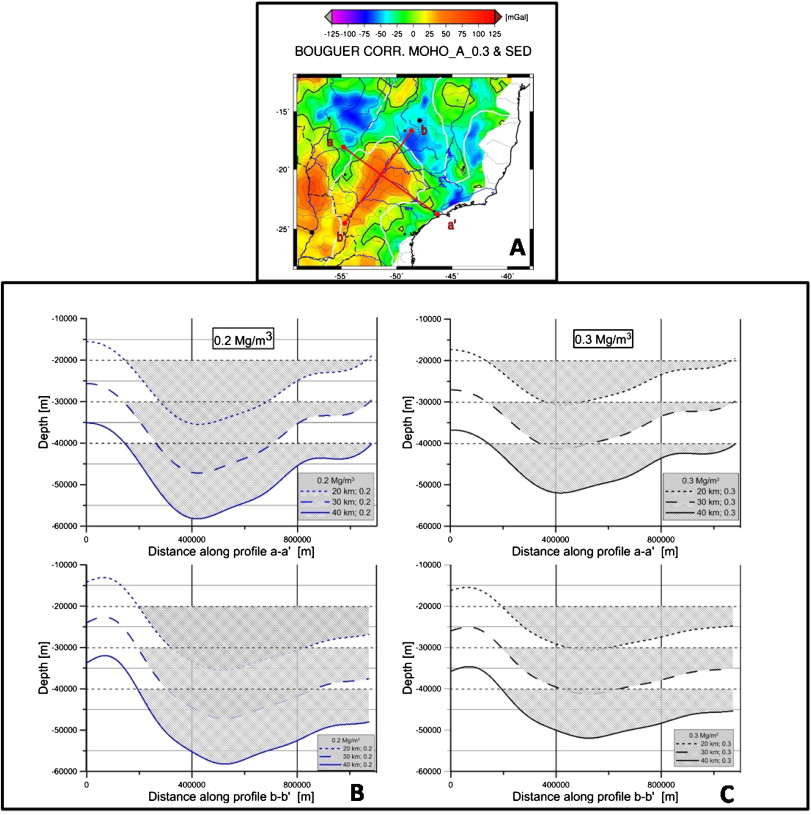
\includegraphics[width=0.8\textwidth]{figures/underplating}
  \end{center}
  \caption{
   Underplating models with a $0.2Mg/m^3$ and $0.3Mg/m^3$ density contrasts for the Paraná Basin, South America. The models are calculated through inversion of gravity data. After \cite{Mariani2013}.
  }
  % Label used to reference the figure in the text.
  \label{fig:underplating}
\end{figure}
The values ultimately used here map out a square intrusion with a density contrast of 200kg/$m^3$ and a depth of -30km to -45km, the lateral extent of this underplating is from -55 to -49 degrees for the west and east longitude points respectively and -27 to -21 degrees for the north and south latitude dimensions. Adding this in should increase the Moho depth in the area, however, the most likely outcome is that it will increase the MSE averages reached in the cross-validation procedure. Although, it is an interesting avenue in calculating and adding previously unmodelled masses into models hopefully increasing the accuracy of gravitationally derived models.
\section{Software Implementation}
This inversion and error estimation method put forward in the methodology is executed in the Python programming language. Software is available under the BSD 3 clause open-source software license. The code in this project depend on open-source libraries scipy and numpy \citep{Harris2020} for number computations, matplotlib (\cite{Hunter2007}, \url{http://matplotlib.org}) and seaborn (\cite{Waskom2015}, \url{https://github.com/mwaskom/seaborn/tree/v0.6.0}) for plots and maps, Fatiando a Terra (\cite{Uieda2013a}, \url{http://www.fatiando.org}) for geophysics tasks. scipy.sparse package is implemented for use on sparse matrix arithmetic and linear algebra and solves the linear equation system equation.
The use of Jupyter notebooks (\cite{Perez2007}, \url{http://jupyter.org/}), which merge the source code, results, and figures of the project.
All source code, Jupyter notebooks, data, and error estimate results are available through an online repository (\url{https://github.com/compgeolab/moho-uncertainty}).
  \chapter{Results and Discussion}

This is where you present the results and discuss their meaning.

  \chapter{Summary}

Conclusion of your dissertation. Summarize what was learned and why it's
relevant.


  \pagestyle{plain}

  % Use the American Geophysical Union citation style
  \bibliographystyle{agu}
  % Use References instead of Bibliography (the default)
  \renewcommand{\bibname}{References}
  % The References section is automatically populated from the cited entries of
  % the references.bib file
  \bibliography{references}

  % If you want to have an appendix, uncomment these two lines and add an
  % appendix.tex file with the text. Sections declared in it will automatically
  % be numbered differently.

  %\appendix
  %\chapter{Appendix}

In order to create the plots and calculate results for this project we had to produce code through python language software in Jupyter lab. The repositories used were saved into the Github page Computer-Oriented Geoscience Lab ``compgeolab'' with the ones which provided all data presented named and described below:
\\ \footnotesize
\\
data/MarsTopo719.shape - Topography data file \\
data/gmm3\_120\_sha.tab - Gravity data file\\
environment.yml -directory that contains the collection of conda packages installed \\
prepare-gravity-grids.ipynb - Code required in order to export the now usable grids to a netCDF file \\
functions.py - Contains the utility functions for this project \\
mars-bouguer-density.ipynb - Code used to performed the calculations plotting figures for all regions used \\
Further-analysed-density.ipynb - Code used for plotting the figures whch were further analysed \\

\normalsize In order to test our code to see if the calculations would acquire an accurate density value we recreated the results of Carartori Tontini [2007]. 
\begin{figure}[H]
	\centering
	\subfloat{\includegraphics[width=65mm]{Figures/Caratori Tontini Recreation}\label{fig:C T recreation}}
	\subfloat{\includegraphics[width=71mm]{Figures/Density from Caratori Tontini}\label{fig:Density from C T}}
\end{figure}
The plots created obtained density value of $2300 kg/m^3$. This is slightly less than the $2400 kg/m^3$ from the paper but, this could be a consequence of using our gravity grid at a height of 10 km instead of 0 km. Despite that it does represent that to calculation performed in the code is successful in finding an accurate optimal Bouguer density; therefore, we can have confidence in the results shown in this Thesis.


\end{document}
